\documentclass[a3paper]{article}
\usepackage[hyphens]{url}
\usepackage[utf8]{inputenc}
\usepackage[pdftex]{graphicx}
\usepackage{epstopdf}
\usepackage{amsmath}
\usepackage{amssymb}
\usepackage{mathrsfs}
\usepackage{booktabs}
\usepackage[ruled,linesnumbered]{algorithm2e}
\usepackage{cleveref}
\usepackage[misc]{ifsym}
\usepackage{longtable}
\urlstyle{same}
\usepackage[a4paper, total={7in, 10in}]{geometry}
\usepackage{amsmath}
\usepackage{amssymb}
\usepackage{cleveref}
\usepackage{booktabs}
\usepackage[switch]{lineno} 
\usepackage{ntheorem}

\usepackage{float}
\restylefloat{table}

\newtheorem{theorem}{Theorem}
\newtheorem{lemma}{Lemma}
\newtheorem*{proof}{\it{Proof.}\rm}

\newcommand{\IE}{\textit{i.e.}, }
\newcommand{\EG}{\textit{e.g.}, }
\newcommand{\ET}{\textit{et al.}}
\newcommand{\ST}{\textit{s.t.}}

\newcommand{\dd}{\mathrm{d}}
\newcommand{\vv}[1]{\bm{\mathrm{{#1}}}}
\newcommand{\E}{\operatorname{\mathbb{E}}}
\newcommand{\EE}[1]{\operatorname{\mathbb{E}}\left[{#1}\right]}
\newcommand{\EEE}[2]{\operatorname{\mathbb{E}}_{{#1}}\left[{#2}\right]}
\newcommand{\KLD}{\operatorname{KL}}
\newcommand{\KLDD}[2]{\operatorname{KL}\left[{#1}\,\big\|\,{#2}\right]}
\newcommand{\abs}[1]{\left|#1\right|}
\newcommand{\Entropy}{\operatorname{H}}
\newcommand{\Entropyy}[1]{\operatorname{H}\left[#1\right]}
\newcommand{\pin}{p_{in}}
\newcommand{\pout}{p_{out}}
\newcommand{\pmix}{p_{mix}}
\newcommand*{\QED}{\hfill\ensuremath{\square}}  %自定义,空心
% Following comment is from ijcai97-submit.tex:
% The preparation of these files was supported by Schlumberger Palo Alto
% Research, AT\&T Bell Laboratories, and Morgan Kaufmann Publishers.
% Shirley Jowell, of Morgan Kaufmann Publishers, and Peter F.
% Patel-Schneider, of AT\&T Bell Laboratories collaborated on their
% preparation.

% These instructions can be modified and used in other conferences as long
% as credit to the authors and supporting agencies is retained, this notice
% is not changed, and further modification or reuse is not restricted.
% Neither Shirley Jowell nor Peter F. Patel-Schneider can be listed as
% contacts for providing assistance without their prior permission.

% To use for other conferences, change references to files and the
% conference appropriate and use other authors, contacts, publishers, and
% organizations.
% Also change the deadline and address for returning papers and the length and
% page charge instructions.
% Put where the files are available in the appropriate places.


\title{Technique Appendix}
\begin{document}

\pagestyle{plain} 

\newpage
\appendix

\section{Counter-examples}

\begin{figure}[H]
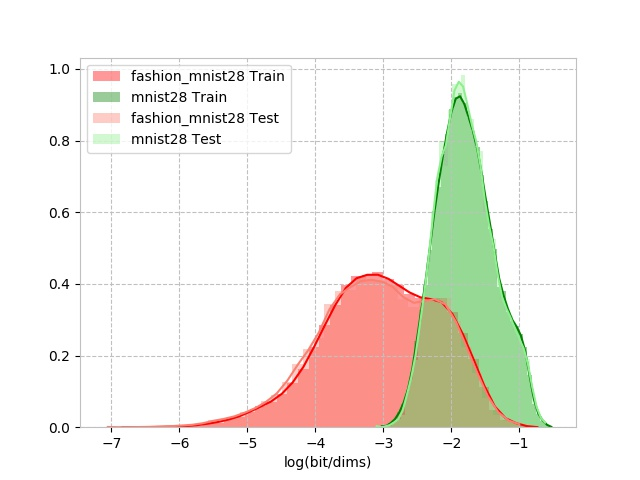
\includegraphics[width=0.5\columnwidth]{figures/log_prob_histogram}
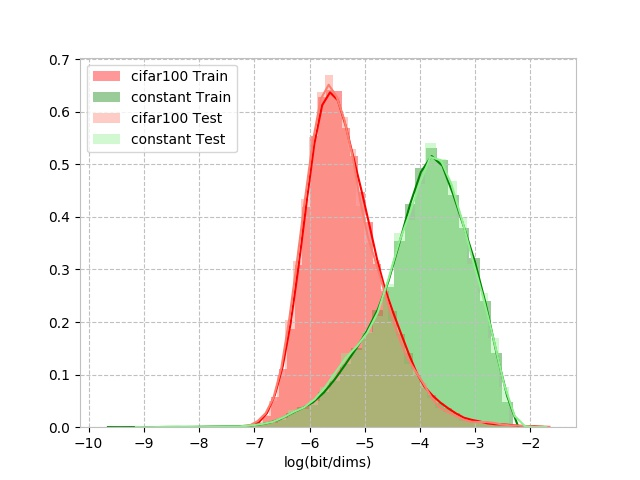
\includegraphics[width=0.5\columnwidth]{figures/log_prob_histogram-1}
\caption{Counter example of $\log p_\theta(x)$ with AUROC 0.0609 and 0.1104}
\end{figure}

\begin{figure}[H]
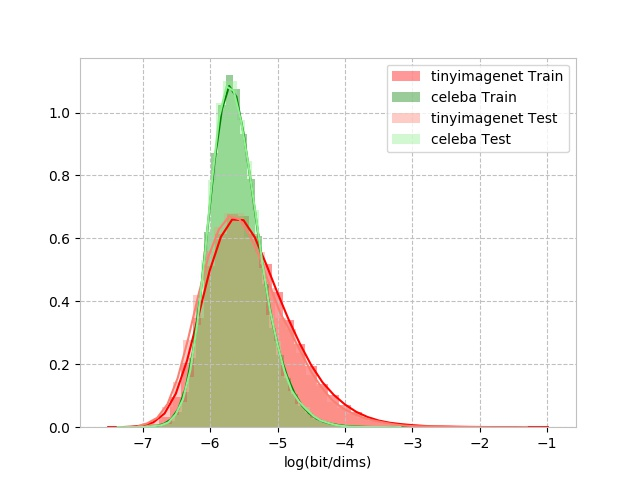
\includegraphics[width=0.5\columnwidth]{figures/log_prob_histogram-3}
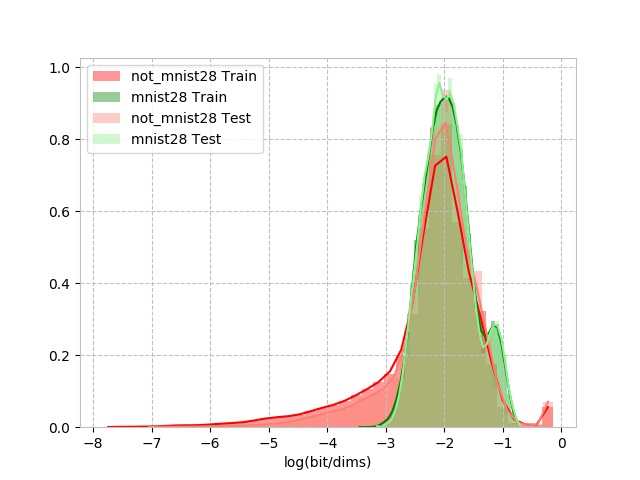
\includegraphics[width=0.5\columnwidth]{figures/log_prob_histogram-4}
\caption{Counter example of $T_{perm}(x)$ with AUROC 0.3933 and 0.4692}
\end{figure}

\begin{figure}[H]
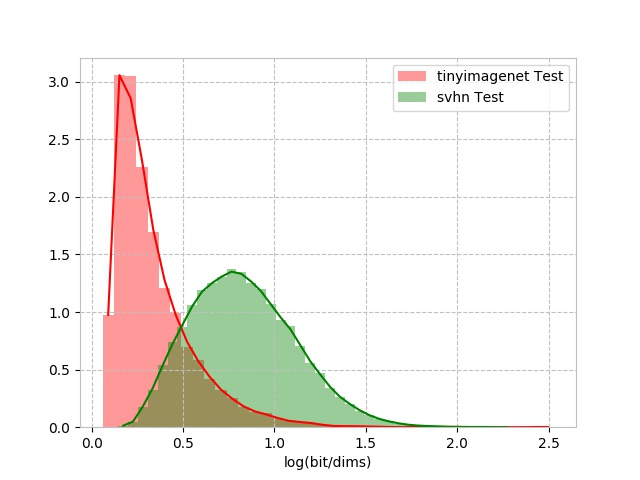
\includegraphics[width=0.5\columnwidth]{figures/grad_norm_histogram}
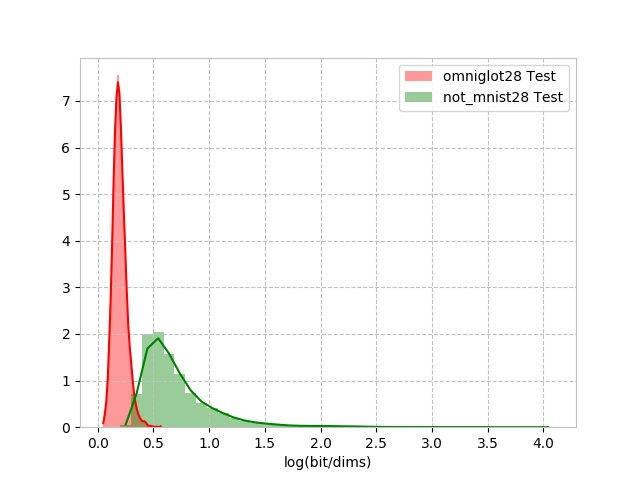
\includegraphics[width=0.5\columnwidth]{figures/grad_norm_histogram-1}
\caption{Counter example of $\|\nabla_x \log p_\theta(x)\|$ with AUROC 0.0196 and 0.0023}
\end{figure}

\begin{figure}[H]
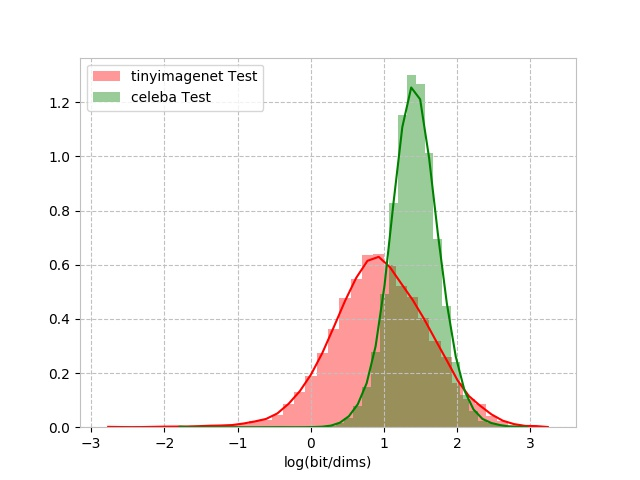
\includegraphics[width=0.5\columnwidth]{figures/ll_with_complexity_histogram}
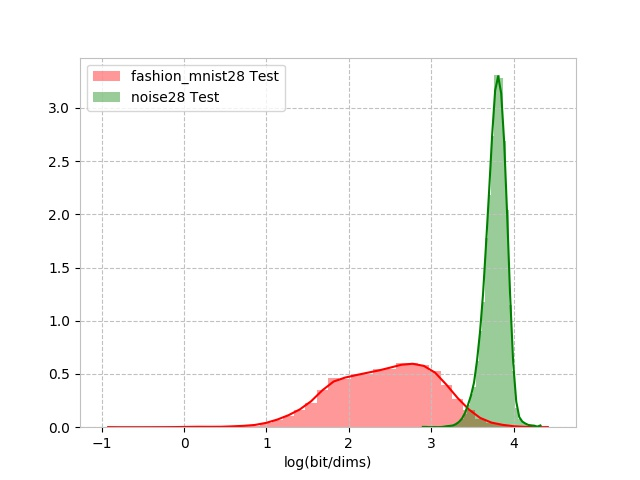
\includegraphics[width=0.5\columnwidth]{figures/ll_with_complexity_histogram-1}
\caption{Counter example of $S(x)$ with AUROC 0.2636 and 0.0062}
\end{figure}


\begin{figure}[H]
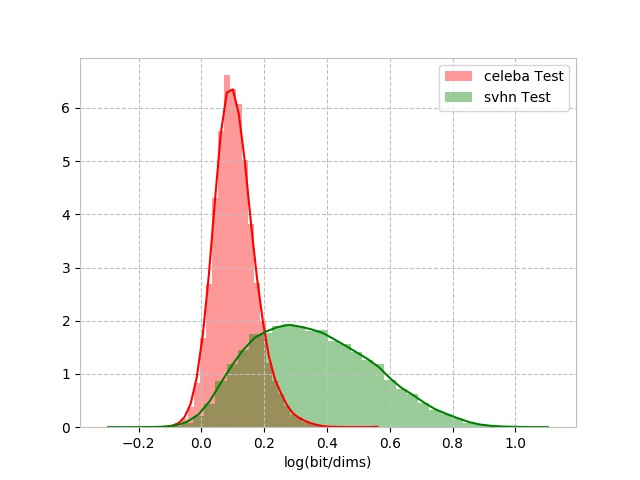
\includegraphics[width=0.5\columnwidth]{figures/kl_histogram}
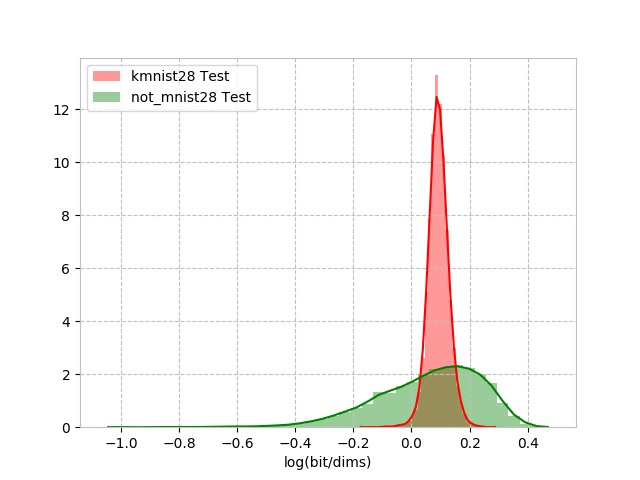
\includegraphics[width=0.5\columnwidth]{figures/kl_histogram-1}
\caption{Counter example of $LLR(x)$ with AUROC 0.1054 and 0.5143}
\end{figure}

\begin{figure}[H]
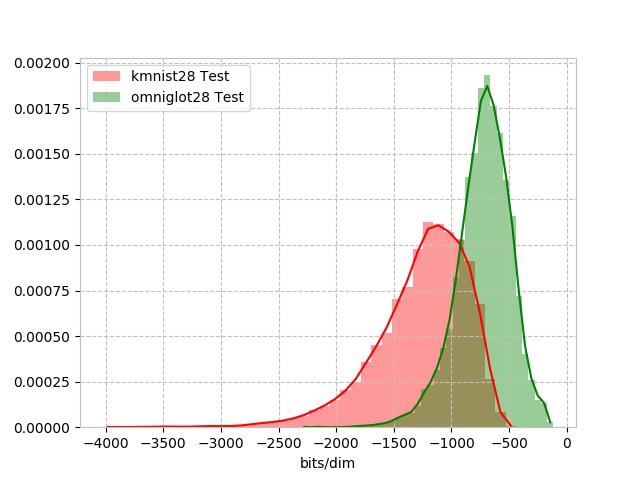
\includegraphics[width=0.5\columnwidth]{figures/ll_waic_histogram}
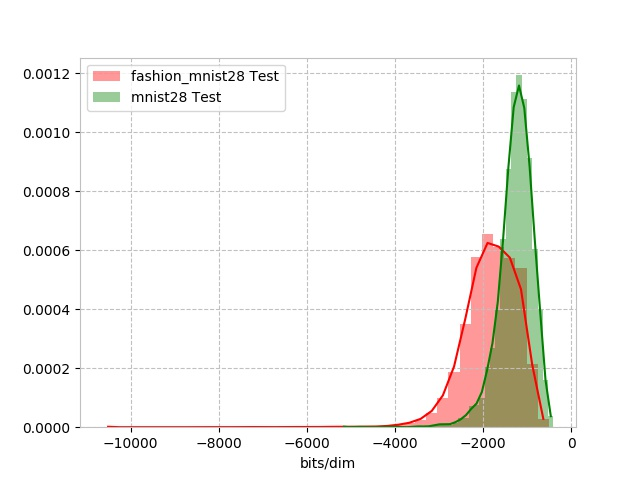
\includegraphics[width=0.5\columnwidth]{figures/ll_waic_histogram-1}
\caption{Counter example of $WAIC(x)$ with AUROC 0.1041 and 0.2135}
\end{figure}

\begin{figure}[H]
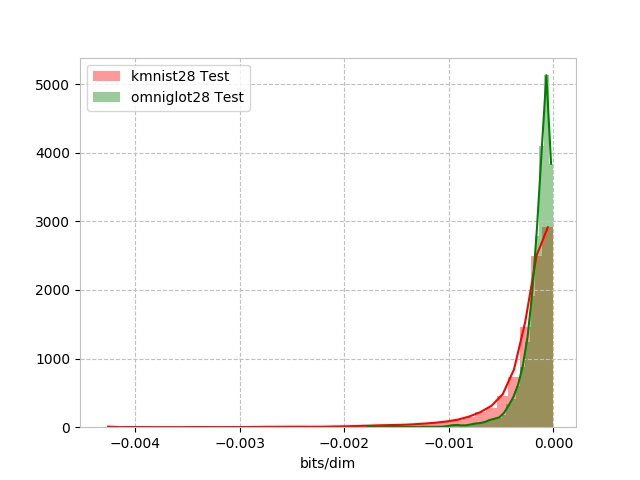
\includegraphics[width=0.5\columnwidth]{figures/var_log_prob_histogram}
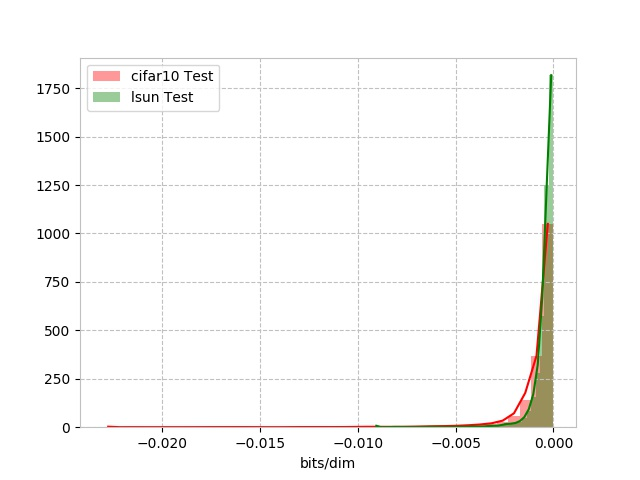
\includegraphics[width=0.5\columnwidth]{figures/var_log_prob_histogram-1}
\caption{Counter example of $\mathop{VAR}_\theta \log p_\theta(x)$ with AUROC 0.5358 and 0.3756}
\end{figure}

\begin{figure}[H]
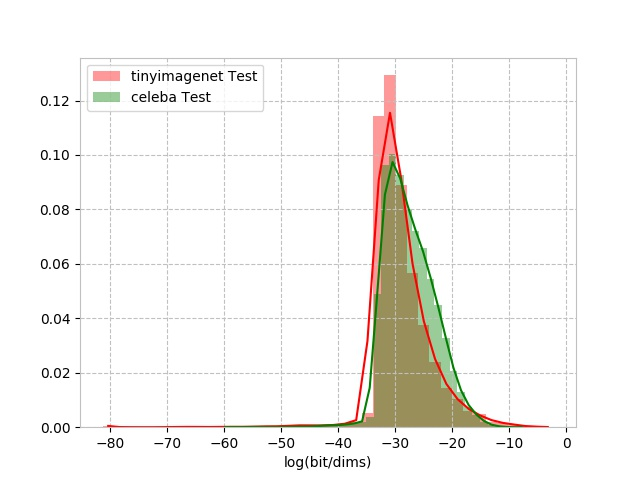
\includegraphics[width=0.5\columnwidth]{figures/log_prob_histogram-5}
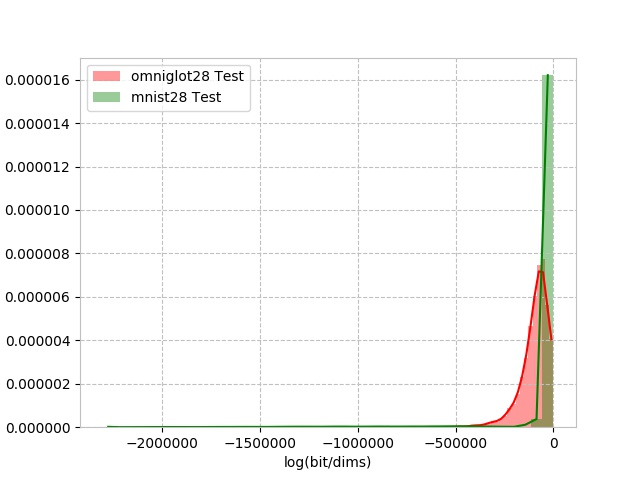
\includegraphics[width=0.5\columnwidth]{figures/log_prob_histogram-6}
\caption{Counter example of $\log p_\theta(x|y)$ with AUROC 0.3822 and 0.1150}
\end{figure}


\section{Experiments}~\label{app:b}

\subsection{Datasets}
%All the datasets considered are listed below:
%\textbf{CIFAR-10}~\cite{krizhevsky2009learning} is a natural image datasets with 10 classes including animal, ship, airplane and etc.
%\textbf{CIFAR-100}~\cite{krizhevsky2009learning} is just like CIFAR-10, including 100 classes.
%\textbf{SVHN}~\cite{netzer2011reading} includes house numbers from 0 to 9.
%\textbf{CelebA}~\cite{liu2015deep} is a large-scale face attributes dataset.
%\textbf{TinyImageNet} consists of a subset of ImageNet images. It contains 200 different classes.
%\textbf{LSUN} has a testing set of 10 different scenes.
%\textbf{iSUN} is subset of SUN, including 8925 scene images in 899 different scenes.
%\textbf{MNIST} consists of handwritten digits from 0 to 9.
%\textbf{Fashion MNIST} includes 10 kinds of clothes and shoes.
%\textbf{Not MNIST} includes letters from A to J on various typefaces.
%\textbf{KMNIST} includes 10 kinds of Kanji characters.
%\textbf{Omniglot} contains 1623 different handwritten characters from 50 different alphabets.
%\textbf{Noise} is created by uniformly randomly sampling.
%\textbf{Constant} includes images whose pixels have same color.
The following datasets are considered: MNIST~\cite{lecun1998gradient}, FashionMNIST~\cite{xiao2017/online}, KMNIST~\cite{clanuwat2018deep}, NOT-MNIST, Omniglot~\cite{lake2015human}, CIFAR-10~\cite{krizhevsky2009learning}, CIFAR-100~\cite{krizhevsky2009learning}, TinyImagenet~\cite{deng2009imagenet}, SVHN~\cite{netzer2011reading}, iSUN~\cite{xu2015turkergaze}, CelebA~\cite{liu2015deep}, LSUN~\cite{yu2015lsun}, Noise and Constant.

Natural images are resized to 32x32x3 and grey images are 28x28x1. All pair in natural image datasets and all pair in grey image datasets are considered in our experiments. Only CIFAR-10, CIFAR-100 and TinyImageNet are not simply-classified and intuitively they have similar classes. LSUN and iSUN are only used as out-of-distribution. CelebA, Noise and Constant have no labels, and we set random labels from 0 to 9 on them. We end up with 92 dataset pairs.

\subsection{Metrics}
Following standard metrics are adopted to measure the effectiveness of a method in out-of-distribution detection:

\noindent \textbf{AUROC} is the Area Under the Receiver Operating Characteristic curve, a threshold-independent metric~\cite{davis2006relationship} and widely used in OoD domain.
%AUROC can be interpreted as the probability that a sample from in-distribution is assigned a lower detection score than a sample from out-of-distribution~\cite{fawcett2006introduction}. It is widely applied in OoD domain. We select AUROC as our major metrics.


\noindent \textbf{AP} is the Average Precision, summarizing the precision-recall curve as the weighted mean of precisions.

\noindent \textbf{FPR@TPR95} is the False Positive Rate when True Positive Rate is over 95\%., which means the probability that an out-of-distribution example is misclassified as in-distribution when over 95\% in-distribution is detected accurately.

\noindent \textbf{AUPR} is the Area under the Precision-Recall curve, which is also threshold independent~\cite{saito2015precision}. % AUPR-In and AUPR-Out denotes the AUPR where in-distribution and out-of-distribution are positive, respectively.


\subsection{Setups}
For fair comparison, all indicators are based on common models with standard training as their proposers suggest, including ResNet34, VAE, PixelCNN, RealNVP. ResNet34 validates whether two datasets are simply-classified and serves for the OoD indicators based on classifier.

In our experiments, there is no validation set. For indicators depending on hyper-parameters, we try grid-searching as their proposers suggest and report the performance with all hyper-parameters considered. To ensure the generality on all datasets, it is forbidden to specify the hyper-parameters or architectures on special dataset.

Our experiments are running on 18 Nvidia GTX 2080Ti of 3 GPU servers. The detailed setup is described in `supplemental/code/README'.  
\subsection{Architecture}
The architecture of VAE is: 

\begin{table}[H]
\centering
\begin{tabular}{lllllll}
Layer     & Channel & Stride & Kernel & Activation  \\
\toprule
Resnet & 16 & 1x1 & 3x3 & Leaky ReLU \\
Resnet & 32 & 1x1 & 3x3 & Leaky ReLU \\
Resnet & 64 & 1x1 & 3x3 & Leaky ReLU \\
Resnet & 128 & 2x2 & 3x3 & Leaky ReLU \\
Resnet & 128 & 2x2 & 3x3 & Leaky ReLU \\
Resnet & 128 & 2x2 & 3x3 & Leaky ReLU \\
Flatten & \\
Dense & 256 &  &  & None \\
\bottomrule
\end{tabular}
\caption{Encoder architecture of VAE}
\end{table}

Before the decoder, we will use dense layer to map $z$ to a tensor with shape $8hw$ and reshape $(h / 4, w / 4, 128)$ where $h, w$ is the height and width of data. 

\begin{table}[H]
\centering
\begin{tabular}{lllllll}
Layer     & Channel & Stride & Kernel & Activation  \\
\toprule
Resnet Deconv & 128 & 2x2 & 3x3 & Leaky ReLU \\
Resnet Deconv & 128 & 2x2 & 3x3 & Leaky ReLU \\
Resnet Deconv & 128 & 2x2 & 3x3 & Leaky ReLU \\
Resnet Deconv & 64 & 1x1 & 3x3 & Leaky ReLU \\
Resnet Deconv & 32 & 1x1 & 3x3 & Leaky ReLU \\
Resnet Deconv & 16 & 1x1 & 3x3 & Leaky ReLU \\
Conv2d & 3 or 1 & 1x1 & 1x1 & None \\
\bottomrule
\end{tabular}
\caption{Decoder architecture of VAE}
\end{table}
We apply a Discretized Logistic Distribution as $p_\theta(x|z)$ and gaussian as $q_\phi(z|x)$. 


The architecture of PixelCNN is: 

\begin{table}[H]
\centering
\begin{tabular}{lllllll}
Layer     & Channel & Vertical Kernel & Horizontal Kernel& Activation & Dropout  \\
\toprule
Resnet & 64 & 2x3 & 2x2 & Leaky ReLU & 0.2\\
Resnet & 64 & 2x3 & 2x2 & Leaky ReLU & 0.2\\
Resnet & 64 & 2x3 & 2x2 & Leaky ReLU & 0.2\\
Resnet & 64 & 2x3 & 2x2 & Leaky ReLU & 0.2\\
Resnet & 64 & 2x3 & 2x2 & Leaky ReLU & 0.2\\
Resnet & 256 & 2x3 & 2x2 & Leaky ReLU & 0.2\\
Flatten & \\
Dense & 256 &  &  & None \\
\bottomrule
\end{tabular}
\caption{Architecture of PixelCNN}
\end{table}


The architecture of Wasserstein is: 

\begin{table}[H]
\centering
\begin{tabular}{lllllll}
Layer     & Channel & Stride & Kernel & Activation  \\
\toprule
Resnet Deconv & 128 & 2x2 & 3x3 & Leaky ReLU \\
Resnet Deconv & 128 & 2x2 & 3x3 & Leaky ReLU \\
Resnet Deconv & 128 & 1x1 & 3x3 & Leaky ReLU \\
Resnet Deconv & 64 & 1x1 & 3x3 & Leaky ReLU \\
Resnet Deconv & 32 & 1x1 & 3x3 & Leaky ReLU \\
Resnet Deconv & 16 & 1x1 & 3x3 & Leaky ReLU \\
Conv2d & 1 & 1x1 & 1x1 & None \\
\bottomrule
\end{tabular}
\caption{Generator architecture of WGAN}
\end{table}

\begin{table}[H]
\centering
\begin{tabular}{lllllll}
Layer     & Channel & Stride & Kernel & Activation  \\
\toprule
Resnet & 16 & 1x1 & 3x3 & Leaky ReLU \\
Resnet & 32 & 1x1 & 3x3 & Leaky ReLU \\
Resnet & 64 & 1x1 & 3x3 & Leaky ReLU \\
Resnet & 128 & 1x1 & 3x3 & Leaky ReLU \\
Resnet & 128 & 2x2 & 3x3 & Leaky ReLU \\
Resnet & 128 & 2x2 & 3x3 & Leaky ReLU \\
\bottomrule
\end{tabular}
\caption{Discriminator architecture of WGAN}
\end{table}

RealNVP has 3 level and 6 blocks at each level. Channel is 128 and activation is ReLU in each block. 
The average runtime memory of VAE, PixelCNN, WGAN and Glow are 2.949GB, 2.851GB, 2.826GB and 2.917GB. 

\subsection{Data-augmentation and steps}
In single-shot fine-tune, the image is randomly shifted in -10\% to 10\% vertically and horizontally, and rotated in -60 to 60 degree, as basic data-augmentation.

The other data-augmentations, containing shifting, rotation, blur, noise, scale, cropping, flipping and modifying contrast and lightness are shown in the following. As can be seen, their performance has no significant difference ($\leq 0.3$\%) to the basic data-augmentation containing rotation and shift. If do not use data-augmentation, fine-tuning is easy to fail (\EG some parameters becomes NaN during fine-tuning). 

\begin{table}[t]
	\centering
	\begin{tabular}{lll}
		\toprule
		Data-augmentation & AUROC \\
		Basic & 95.2470\\
		+Flip & 95.3480\\
		+Crop & 95.1940\\
		+Blur & 95.2464\\
		+Noise & 95.4416\\
		+Contrast & 95.2464\\
		+Light & 95.2680\\
		+Scale & 95.3076\\
		\bottomrule
	\end{tabular}
	\caption{Ablation study about data-augmentations. }
\end{table}

In single-shot fine-tune, the number of steps influence the performance, as shown in the following.

\begin{figure}
\centering
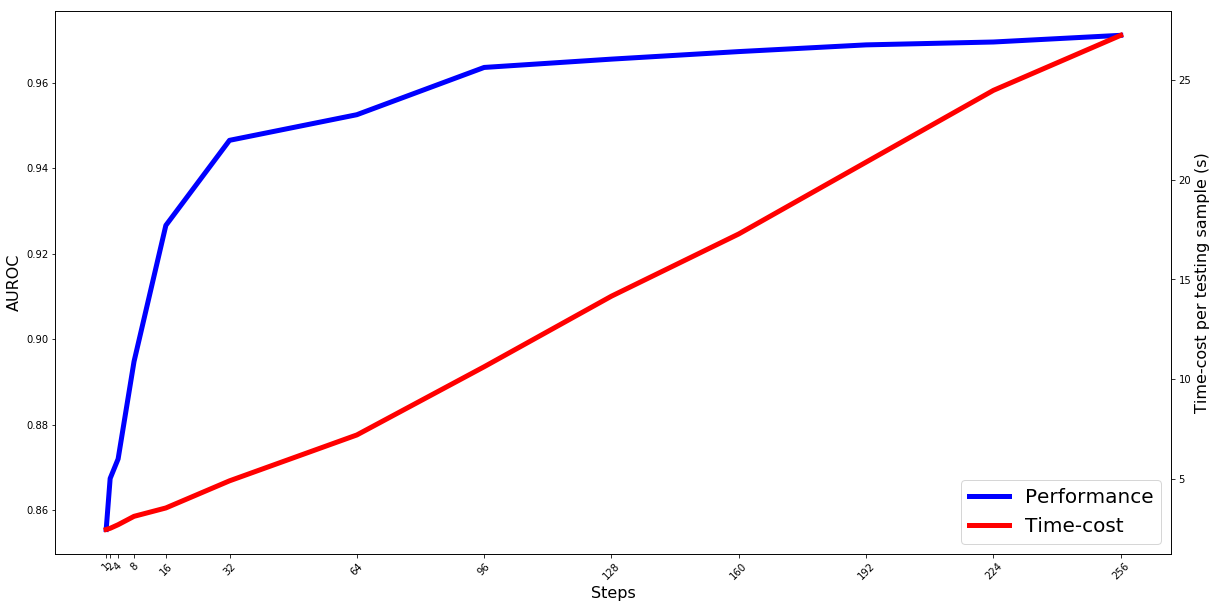
\includegraphics[width=\textwidth]{auroc_steps}	
\caption{The AUROC when step is from 1 to 256. When step is less than 64, step significant influence the AUROC, and when step is larger than 64, AUROC is nearly same. Therefore, we set step = 64 as the default parameter of single-shot fine-tune. Additional, when step =64, the time-cost is only 7s per testing sample.}
\end{figure}


%The hyper-parameters for VAE, PixelCNN, WGAN and Glow are shown in the scripts, shown in code appendix. 
%The detailed experiments are shown in appendix D. 

\section{Theorem}~\label{app:c}

We will derive the theorems in our papers by the assumptions:

\noindent \textbf{1.} $D^{train}_{in}, D^{test}_{in}$ are i.i.d. from distribution $\pin$ and $D^{test}_{out}, D^{train}_{out}$ are i.i.d. from distribution $\pout$.

\noindent \textbf{2.}  $div$ is a divergence , satisfying that $div(\pin, \pout) \gg 0$ and $div(\pout, \pin) \gg 0$.

\noindent \textbf{3.}  If $div(\pin, \pout)$ and $div(\pout, \pin)$ can be represented by sampling formula, \IE $div(\pin, \pout) \approx \sum_{i} f(x_i)$, then $f(x_i) \gg 0$ for most $x_i$ in $\pin$.

\noindent \textbf{4.} $f: \mathcal{X} \rightarrow \mathcal{R}$ maps the distribution $\pin, \pout$ into two Gaussian distribution with constant variance.

\noindent \textbf{5.} Assumption 3 and 4 hold for any $\hat{f}$ approximating $f$.

\textbf{Lemma 1.}\textit{
	Indicators $f_0$ and $f_1$ satisfying that if $f_0(x_1) < f_0(x_2)$ then $f_1(x_1) < f_1(x_2)$ and if $f_0(x_1) > f_0(x_2)$ then $f_1(x_1) > f_1(x_2)$ for $x_1, x_2$ in mixture distribution, have same performance for OoD. We call $f_0 \triangleq f_1$. 
}

\begin{proof}\rm
	Assume we get data $x_0, x_1, \ldots, x_n$ from mixture distribution. The metrics AUROC, AUPR, FPR@TPR95 and AP for indicator $f$ are all dependent on the order of $f(x_0), f(x_1), \ldots, f(x_n)$. The array $f_0(x_0), f_0(x_1), \ldots, f_0(x_n)$ and $f_1(x_0), f_1(x_1), \ldots, f_1(x_n)$ have the same order and then they have same performance for all metrics considered in OoD. 
\end{proof}

\begin{theorem}~\label{thm1}
	$\log \pin(x) - \log \pout(x)$ and $\log p_\theta(x) - \log p_\omega(x)$ and are effective symmetric indicators, \IE it reaches same performance in experiment A vs B and B vs A, with threshold 0, where $p_\theta \rightarrow \pin$ and $p_\omega \rightarrow \pout$. $\log p_\theta(x)$ maps $\pin$ into a gaussian distribution. 
\end{theorem}

\begin{proof}\rm
	We select $KL$ as $div$. By assumption 3 and 4, we have
	\begin{equation*}
		\log \pin(x_1) - \log \pout(x_1) \gg 0 \quad and \quad \log \pin(x_2) - \log \pout(x_2) \ll 0 
	\end{equation*}
	where $x_1 \sim \pin$ and $x_2 \sim \pout$. By assumption 5, above equation holds for $\log p_\theta(x) - \log p_\omega(x)$. Therefore, $\log \pin(x) - \log \pout(x)$ and $\log p_\theta(x) - \log p_\omega(x)$ can detect most of OoD, with threshold zero. 
	
	In experiment A vs B and B vs A, the indicator is $\log p_A(x) - \log p_B(x)$ and $\log p_B(x) - \log p_A(x)$. These two experiments have same mixture distribution. For any testing data $x_1, x_2$ in mixture distribution, if $\log p_A(x_1) - \log p_B(x_1) > \log p_A(x_2) - \log p_B(x_2)$, then $\log p_B(x_1) - \log p_A(x_1) < \log p_B(x_2) - \log p_A(x_2)$. Conversely, if $\log p_A(x_1) - \log p_B(x_1) < \log p_A(x_2) - \log p_B(x_2)$, then $\log p_B(x_1) - \log p_A(x_1) > \log p_B(x_2) - \log p_A(x_2)$. Thus, they have inverse order. 
	Noting that the positive and negative labels in experiment A vs B and B vs A are also inverse, $\log \pin(x) - \log \pout(x)$ reaches same performance in experiment A vs B and B vs A. The proof for $\log p_\theta(x) - \log p_\omega$ is the same as above. 
	
	Let $f(x) = \log \pin(x)$ and $\hat{f}(x) = \log p_\theta(x)$. Since $p_\theta \rightarrow \pin$, $\hat{f} \rightarrow f$. By assumption 4,5, we know $\hat{f} = \log p_\theta(x)$ maps $\pin$ into a gaussian distribution. 
\end{proof}

\begin{theorem}~\label{thm2}
	For any mixture distribution $\pmix = \alpha \pin + \beta \pout$ where $\alpha + \beta = 1$ and $\alpha, \beta > 0$, the performance of indicator $\log \pin(x) - \log \pmix(x)$ and indicator $\log \pin(x) - \log \pout(x)$ is equal for OoD detection. 
\end{theorem}

\begin{proof}\rm
	For any $x1,x2$ satisfying $\log \pin(x_1) - \log \pout(x_1) < \log \pin(x_2) - \log \pout(x_2)$, we have $\log \pin(x_1) - \log \pmix(x_1) < \log \pin(x_2) - \log \pmix(x_2)$ by
	\begin{align*}
		&\log \pin(x) - \log \pmix(x) = -\log \frac{\alpha \pin(x) + \beta \pout(x)}{\pin(x)} = -\log 
		\Big(\alpha + \beta \frac{\pout(x)}{\pin(x)}\Big) \\
		&\log \frac{\pin(x_1)}{\pout(x_1)} < \log \frac{\pin(x_2)}{\pout(x_2)} \Rightarrow \frac{\pin(x_1)}{\pout(x_1)} < \frac{\pin(x_2)}{\pout(x_2)} \Rightarrow \frac{\pout(x_1)}{\pin(x_1)} > \frac{\pout(x_2)}{\pin(x_2)} \\
	 &\Rightarrow \log \Big(\alpha + \beta \frac{\pout(x_1)}{\pin(x_1)}\Big) > \log 
		\Big(\alpha + \beta \frac{\pout(x_2)}{\pin(x_2)}\Big) \\
		&\Rightarrow -(\log \pin(x_1) - \log \pmix(x_1)) > -(\log \pin(x_2) - \log \pmix(x_2)) \\
		&\Rightarrow \log \frac{\pin(x_1)}{\pmix(x_1)} < \log \frac{\pin(x_2)}{\pmix(x_2)} 
	\end{align*}
	
	By the same way, for any $x1,x2$ satisfying $\log \pin(x_1) - \log \pout(x_1) > \log \pin(x_2) - \log \pout(x_2)$, we have $\log \pin(x_1) - \log \pmix(x_1) > \log \pin(x_2) - \log \pmix(x_2)$.  By \cref{lemma1}, performance of indicator $\log \pin(x) - \log \pmix(x)$ and indicator $\log \pin(x) - \log \pout(x)$ is equal for OoD detection.
	
	\noindent \textbf{Remark.} In the proof, we do not use the condition that $\alpha > 0$ but only $\beta > 0$ and $\pmix(x) > 0$. It means that \cref{thm2} holds even when $\alpha < 0, \beta > 0$ and $\pmix(x) > 0$. 
\end{proof}


\begin{theorem}~\label{thm3}On any dataset pair that log-likelihood works well, \IE $\log \pin(x_1) > \log \pin(x_2)$ for most $x_1 \sim \pin, x_2 \sim \pout$, KL-based indicator can reach better performance.
\end{theorem}

\begin{proof}\rm
	Noting that the AUROC is related to the Mann–Whitney U, which tests whether positives are ranked higher than negatives, whose number called distortion. 
	For each $x_1 \sim \pin, x_2 \sim \pout$,
	assume $\log \pout(x_1) < \log \pout(x_2)$, then $\log \pin(x_1) - \log \pout(x_1) > \log \pin(x_2) - \log \pout(x_2)$. 
	KL-based indicator will get same performance than log-likelihood indicator. 
	
	Assume $\log \pout(x_1) > \log \pout(x_2)$, then likelihood indicator will make mistake in experiment B vs A (if current experiment is A vs B). Meanwhile KL-based indicator might detect OoD in both A vs B and B vs A by \cref{thm1}. In conclusion, likelihood leads to more distortion than KL-based indicator, in experiment B vs A and experiment A vs B.
	
	It means KL-based indicator is always better than log-likelihood indicator. 
\end{proof}

For the proofing of following theorems, we need an additional mathematical simplification: by assumption 4 and 5, the indicators for OoD maps the distribution $\pin, \pout$ into two Gaussian distribution with constant variance, therefore, the AUROC between these two Gaussian distribution is dependent on the difference of their mean, \IE $\E_{\pin(x)} f(x) - \E_{\pout(x)} f(x)$ is our simplified metric for mathematical inference. 



\begin{theorem}~\label{thm4}
For any likelihood-ratio indicator $\log \pin(x) - \log g(x)$ where $g$ is a continuous differentiable probability distribution, KL-based indicator outperforms them.
\end{theorem}
\begin{proof}\rm
	Consider the following optimization with subsidiary conditions for searching the optimal $g$ for likelihood ratio:
	\begin{align*}
	\max_g \Big\{\E_{\pin(x)} \big[\log \pin(x) - \log g(x)\big] &- \E_{\pout(x)} \big[\log \pin(x) - \log g(x)\big]\Big\} \\
	\textbf{s.t.} KL(\pin, g) = L \text{ and } &\int g(x) \dd x = 1 
	\end{align*}
	where $L$ is a constraint to the optimization domain of $g$. It could be solved by Lagrange multiplier method introduced by calculus of variation. 
	Let $\lambda, \psi > 0$ be Lagrange Multiplier for the two constraint. The Lagrange function is 
	\begin{align*}
		J[g] &= \E_{\pin(x)} \big[\log \pin(x) - \log g(x)\big] - \E_{\pout(x)} \big[\log \pin(x) - \log g(x)\big] \\
		&-\lambda KL(\pin, g) - \psi \int g(x) \dd x \\
		&= \int \pin(x) \log \pin(x) - \pin(x) \log g(x) - \pout(x) \log \pin(x) \\ 
		&+ \pout(x) \log g(x) - \lambda \pin(x) \log \frac{\pin(x)}{g} - \psi g(x) \dd x = \int F(g, x) \dd x
	\end{align*}
	By calculus of variation, the extremal point for $J[g]$ satisfies that $\delta J = 0$, which is equal to
	\begin{align*}
		\frac{\partial F(g, x)}{\partial g} = 0 \Rightarrow -\frac{\pin(x)}{g(x)} + \frac{\pout(x)}{g(x)} + \frac{\lambda \pin(x)}{g(x)} - \psi = 0 \\
		\Rightarrow g(x) = \frac{1}{\psi} ((\lambda - 1)\pin(x) + \pout(x))
	\end{align*}
	Considering the subsidiary condition $\int g(x) \dd x = 1$, we have
	\begin{equation*}
		\int g(x) \dd x = \frac{1}{\psi} \int (\lambda - 1) \pin(x) + \pout(x) \dd x = \frac{1}{\psi} ((\lambda - 1) + 1) = \frac{\lambda}{\psi} = 1
	\end{equation*}
	Therefore, $\lambda = \psi$ and $g^*(x) = \frac{\lambda - 1}{\lambda} \pin(x) + \frac{1}{\lambda} \pout(x)$ is the extremal point.
	By the remark of \cref{thm1}, $\log \pin(x) - \log g^*(x)$ gets same performance as $\log \pin(x) - \log \pout(x)$ in OoD detection. 
	For any $L$, we can get $g^*(x)$, which has same performance as $\log \pin(x) - \log \pout(x)$. It means that KL-based indicator is the optimal indicator among all likelihood-ratio indicators. 
\end{proof}

\begin{theorem}~\label{thm5}
	$\log \frac{p_\theta(x)}{p_\gamma(x)}$ can reach better AUROC than KL-based indicator, when $p_\gamma$ is well-trained, \IE $p_\gamma$ reaches better likelihood on $\pmix$ than $p_{\hat{\gamma}} = \alpha p_{\theta} + \beta p_{\omega}$. 
\end{theorem}
\begin{proof}\rm
	Let $p_{\hat{\gamma}}(x) = \alpha p_\theta(x) + \beta p_\omega(x)$. $\hat{\gamma}$ is the parameters that can be obtained by optimizer. 
	Considering the indicator $\log p_\theta(x) - \log p_{\hat{\gamma}}(x) = -\log (\alpha + \beta \frac{p_\omega(x)}{p_\theta(x)})$, for $x_1 \sim \pin$ and $x_2 \sim \pout$, we have 
	\begin{align*}
		\log \frac{p_\theta(x_1)}{p_{\hat{\gamma}}(x_1)} - \log \frac{p_\theta(x_2)}{p_{\hat{\gamma}}(x_2)} = \log (\alpha + \beta \frac{p_\omega(x_2)}{p_\theta(x_2)}) - \log (\alpha + \beta \frac{p_\omega(x_1)}{p_\theta(x_1)})
	\end{align*}
	We have known that $\log \frac{p_\theta(x_1)}{p_\omega(x_1)} \gg 0$ and $\log \frac{p_\theta(x_2)}{p_\omega(x_2)} \ll 0$ by \cref{thm1}. Then, we have $\log \frac{p_\theta(x_1)}{p_{\hat{\gamma}}(x_1)} - \log \frac{p_\theta(x_2)}{p_{\hat{\gamma}}(x_2)} > 0$. It means that $\log \frac{p_\theta(x)}{p_{\hat{\gamma}}(x)}$ can be used for detecting OoD.
	
	Next, consider the $\gamma$ is optimized better than $\hat{\gamma}$, \IE $\E_{\pmix} \log p_\gamma(x) \geq \E_{\pmix} \log p_{\hat{\gamma}}(x)$. 
	
	\begin{align*}
		\E_{\pmix} \log p_\gamma(x) = \alpha \E_{\pin} \log p_\gamma(x) + \beta \E_{\pout} \log p_\gamma(x)
	\end{align*}
	By $\E_{\pmix} \log p_\gamma(x) \geq \E_{\pmix} \log p_{\hat{\gamma}}(x)$, there are 3 case:
	
	\textbf{1.} $\E_{\pin} \log p_\gamma(x) \leq \E_{\pin} \log p_{\hat\gamma}(x)$ and $\E_{\pout} \log p_\gamma(x) \geq \E_{\pout} \log p_{\hat\gamma}(x)$. 
	
	\textbf{2.} $\E_{\pin} \log p_\gamma(x) \geq \E_{\pin} \log p_{\hat\gamma}(x)$ and $\E_{\pout} \log p_\gamma(x) \geq \E_{\pout} \log p_{\hat\gamma}(x)$. 
	
	
	\textbf{3.} $\E_{\pin} \log p_\gamma(x) \geq \E_{\pin} \log p_{\hat\gamma}(x)$ and $\E_{\pout} \log p_\gamma(x) \leq \E_{\pout} \log p_{\hat\gamma}(x)$. 
	
	By assumption 4, 5 and simplified metric, we know that if  $\E_{\pin} \log p_\gamma(x)$ increase, the KL-based indicator $\log \frac{p_\theta(x)}{p_{{\gamma}}(x)}$ will be worse and if  $\E_{\pout} \log p_\gamma(x)$ increase, the KL-based indicator $\log \frac{p_\theta(x)}{p_{{\gamma}}(x)}$ will be better. 
	
	Therefore, in case 1, the performance of $\log \frac{p_\theta(x_1)}{p_{\gamma}(x_1)}$ will be better than $\log \frac{p_\theta(x_1)}{p_{\hat\gamma}(x_1)}$. In case 2 and 3, we know $\E_{\pin} \log p_{\hat\gamma}(x) \leq \E_{\pin} \log p_\theta(x)$ and $\E_{\pin} \log p_\gamma(x) \leq \E_{\pin} \log p_\theta(x)$ since $\theta$ is well-trained for such loss function. 
	\begin{align*}
		\beta \E_{\pout} \log p_\gamma(x) = \E_{\pmix} \log p_\gamma(x) - \alpha \E_{\pin} \log p_\gamma(x) \\
		\geq \E_{\pmix} \log p_{\hat\gamma}(x) - \alpha \E_{\pin} \log p_\theta(x) \\
		= \alpha \E_{\pin} \log \frac{p_{\hat \gamma}(x)}{p_\theta(x)} + \beta \E_{\pout} \log p_{\hat \gamma}(x) \\
	\Rightarrow \E_{\pout} \log \frac{p_\gamma(x)}{p_{\hat\gamma}(x)} \geq \frac{\alpha}{\beta} \E_{\pin} \log \frac{p_{\hat \gamma}(x)}{p_\theta(x)}
	\end{align*}
	And we have 
	\begin{equation*}
		\E_{\pin} \log \frac{p_\gamma(x)}{p_{\hat\gamma}(x)} \leq \E_{\pin} \log \frac{p_\theta(x)}{p_{\hat\gamma}(x)}
	\end{equation*}
	Therefore, by our simplified metric, we have
	\begin{align*}
		(\E_{\pin(x)} \log \frac{p_\theta(x)}{p_{{\gamma}}(x)} - \E_{\pout(x)} \log \frac{p_\theta(x)}{p_{{\gamma}}(x)}) - (\E_{\pin(x)} \log \frac{p_\theta(x)}{p_{{\hat\gamma}}(x)} - \E_{\pout(x)} \log \frac{p_\theta(x)}{p_{\hat\gamma}(x)}) \\
		=  \E_{\pout} \log \frac{p_\gamma(x)}{p_{\hat\gamma}(x)} -\E_{\pin} \log \frac{p_{\gamma}(x)}{p_{\hat\gamma}(x)}\geq \frac{\alpha}{\beta} \E_{\pin} \log \frac{p_{\hat \gamma}(x)}{p_\theta(x)} - \E_{\pin} \log \frac{p_\theta(x)}{p_{\hat\gamma}(x)} \\
		= \frac{\alpha + \beta}{\beta} \E_{\pin} \log \frac{p_\theta(x)}{p_{\hat\gamma}(x)} = \frac{1}{\beta} \E_{\pin} \log \frac{p_\theta(x)}{p_{\hat\gamma}(x)} \geq 0
	\end{align*}
	It means that $\frac{p_\theta(x)}{p_{{\gamma}}(x)}$ is a better OoD indicator than $\frac{p_\theta(x)}{p_{{\hat\gamma}}(x)}$ in case 2 and 3. In conclusion,  $\frac{p_\theta(x)}{p_{{\gamma}}(x)}$ will be a better OoD indicator and thus they can be used to detect OoD if $\gamma$ is trained better than $\hat{\gamma}$. 
%	Additional, by the above proof, since $p_\gamma$ is optimized from $p_\theta$, the sign of $\log \frac{p_\theta(x)}{p_\gamma(x)}$ represents whether the likelihood of $x$ in mixture distribution is improved during the mixture training.
	
\end{proof}
%
%\begin{theorem}\label{thm6}
%	Assumption 2 is a corollary of definition of OoD problem when $div$ is Wasserstein distance.
%\end{theorem}
%\begin{proof}
%	By the definition of OoD, exist a $L > 0$, for any $x_1 \sim \pin, x_2 \sim \pout$, their distance $\|x_1 - x_2\|$ is at least $L$. 
%	\begin{equation*}
%		 W^1(\pin, \pout) = \min_{f \in \Gamma(\pin, \pout)} \iint f(x_1, x_2) \|x_1 - x_2\| \dd x_1 \dd x_2 \geq L
%	\end{equation*}
%\end{proof}
%
%\begin{theorem}\label{thm7}
%	$D(x)$ is a symmetric indicator.
%\end{theorem}
%\begin{proof}
%	Let $D$ is the optimal discriminator in $W^1(\pin, \pout)$, for any $D'$ satisfying $Lip(D') \leq 1$, we have
%	\begin{align*}
%		\E_{\pout} D'(x) - \E_{\pin} D'(x) = \E_{\pin} [-D'(x)] - \E_{\pout} [-D'(x)] \\
%		\leq  \E_{\pin} D(x) - \E_{\pout} D(x) =  \E_{\pout} [-D(x)] - \E_{\pin} [-D(x)] 
%	\end{align*}
%	Therefore, $-D(x)$ is the optimal discriminator in $W^1(\pout, \pin)$. By the same way in \cref{thm1}, 
%	$D(x)$ is a symmetric indicator.
%\end{proof}
%
%\begin{theorem}\label{thm8}
%	$\hat{D}$ that is optimal solution in $W^1(\pin, \pmix)$ is same to the optimal solution $D$ in $W^1(\pin, \pout)$. Moreover, the neural networks trained by $W^1(\pin, \pmix)$ and $W^1(\pin, \pout)$ will share the same optimization process.
%\end{theorem}
%
%\begin{proof}
%	For any $D$ satisfying $Lip(D) \leq 1$, 
%	\begin{align*}
%		\E_{\pin} D(x) - \E_{\pmix} D(x) = \E_{\pin} D(x) - \alpha\E_{\pin} D(x) - \beta\E_{\pout} D(x) \\ 
%		= (1 - \alpha)\E_{\pin} D(x) - \beta\E_{\pout} D(x)
%		= \beta \E_{\pin} D(x) - \beta \E_{\pout} D(x) \\
%		\leq \beta \E_{\pin} \hat{D}(x) - \beta \E_{\pout} \hat{D}(x) = (1 - \alpha)\E_{\pin} \hat{D}(x) - \beta\E_{\pout} \hat{D}(x) \\
%		= \E_{\pin} \hat{D}(x) - \alpha\E_{\pin} \hat{D}(x) - \beta\E_{\pout} \hat{D}(x) = \E_{\pin} \hat{D}(x) - \E_{\pmix} \hat{D}(x)
%	\end{align*}
%	Therefore, $\hat{D}$ is also the optimal discriminator in $W^1(\pin, \pmix)$. Additional, in above proof, the loss functions for $D$ in $W^1(\pin, \pmix)$ and $W^1(\pin, \pout)$ are 
%	\begin{equation*}
%		\E_{\pin} D(x) - \E_{\pmix} D(x) = \beta (\E_{\pin} D(x) - \E_{\pout} D(x))
%	\end{equation*}
%	The two loss functions have same gradient direction for neural network optimization, thus the training optimization processes are same.
%\end{proof}
%
%\begin{theorem}\label{thm9}
%	The discriminator in $W^1(\pin, \pout)$ is the best indicator among all indicators that is 1-Lipschitz. Moreover, it is the best indicator who has limited gradient.
%\end{theorem}
%\begin{proof}
%	By our simplified metric, for any indicator $f$, 
%	\begin{equation*}
%		\E_{\pin} f(x) - \E_{\pout} f(x)
%	\end{equation*}
%	measures the performance of OoD detection. Thus 
%	\begin{equation*}
%		\max_{Lip(f) \leq 1} \E_{\pin} f(x) - \E_{\pout} f(x) = W^1(\pin, \pout)
%	\end{equation*} 
%	will search the best indicator among all indicators that is 1-Lipschitz. Especially, for a indicator $f$ has limited gradient $K$, function $g(x) = f(x) / K$ satisfies that $Lip(g) \leq 1$. By \cref{thm1}, $f \triangleq g$, and $g$ is worse than the optimal discriminator in $W^1(\pin, \pout)$. 
%	
%\end{proof}

\section{Detailed Experiments}
See the `detailed\_experiment' in supplemental file. 

%% The file named.bst is a bibliography style file for BibTeX 0.99c



%% The file named.bst is a bibliography style file for BibTeX 0.99c
\bibliographystyle{splncs04}
\bibliography{reference}


\end{document}

